\documentclass[preprint]{sigplanconf}
\usepackage{amsmath,amssymb,amsthm}
\usepackage{color,graphicx,subfigure}
\usepackage{algpseudocode}
\algtext*{EndWhile}% Remove "end while" text
\algtext*{EndIf}% Remove "end if" text
\algtext*{EndFor}% Remove "end for" text
\usepackage{qtree}
\usepackage{epsfig,epstopdf}
\usepackage{multirow}
\usepackage{listings}
\usepackage{url}

\newcommand{\shrink}{\vspace*{-2ex}}

\newcommand{\TODO}[1]{\vspace*{2mm}\textcolor{red}{\fbox{TODO: #1}}\vspace*{2mm}}
\newcommand{\XJ}[1]{\textcolor{red}{[XJ: #1]}}
\newcommand{\KZ}[1]{\textcolor{blue}{[KZ: #1]}}
\newcommand{\RY}[1]{\textcolor{blue}{[RY: #1]}}

\newcommand{\nat}{\mathbb{N}}

\newcommand{\cm}{\mathbf{cm}}
\newcommand{\cu}{\mathbf{cu}}
\newcommand{\exit}{\mathbf{exit}}
\newcommand{\To}{\longrightarrow}
\newcommand{\computes}{\To_p}
\newcommand{\exiting}{\mathbf{exiting}}
\newcommand{\exited}{\mathbf{exited}}

\newcommand{\In}{\mathbf{in}}
\newcommand{\Out}{\mathbf{out}}
\newcommand{\Rd}{\mathbf{rd}}

\newcommand{\dm}{\mathcal{DM}}
\newcommand{\alltype}{\mathcal{T}}
\newcommand{\allop}{\mathcal{P}}
\newcommand{\allstore}{\mathcal{D}}

\newcommand{\typeof}[1]{\tau\ldbrack #1\rdbrack}

\newcommand{\ldbrack}{[\hspace{-0.5mm}[}
\newcommand{\rdbrack}{]\hspace{-0.5mm}]}
\newcommand{\lbb}{\{\hspace{-0.7mm}|}
\newcommand{\rbb}{|\hspace{-0.7mm}\}}

\newcommand{\compact}[1]{\!\!#1\!}
\newcommand{\bk}{\hspace{-1mm}}

\newtheorem{theorem}{Theorem}
\newtheorem{lemma}{Lemma}
\newtheorem{proposition}{Proposition}
\newtheorem{corollary}{Corollary}
\newtheorem{definition}{Definition}
\newtheorem{property}{Property}
\newtheorem{axiom}{Axiom}
\newtheorem{example}{Example}

\newcommand{\figref}[1]{Figure \ref{#1}}
\newcommand{\tabref}[1]{Table \ref{#1}}
\newcommand{\eqnref}[1]{Eq. (\ref{#1})}

\newcommand{\nl}{\vspace*{3mm}}

% \makeatletter
%  \let\@copyrightspace\relax
% \makeatother

\lstset{
  captionpos=b,
  tabsize=2,
  % numbers=left,
  % numberstyle=\tiny,
  % numbersep=5pt,
  breaklines=true,
  showstringspaces=true,
  basicstyle=\scriptsize\ttfamily,
  frame=none,
  emph={label},
  escapechar=| % Escape to LaTeX between |...|
}

\renewcommand{\shrink}{\vspace*{-2ex}}

\title{Speculative Nondeterminism}
\authorinfo{}{}{} % enable double-blind reviewing

\begin{document}

\maketitle

\begin{abstract}
We propose a new programmable concurrency control framework called
speculative nondeterminism for real time,
``open'' and distributed agents. 
%By open, we mean the agent programs
%are independent and are not necessarily constrained to operate
%in a particular fashion, and they may join the system at arbitrary times.
In this framework, dynamic and concurrent agent programs 
affect each other through a centralized store which represents shared resources.
%There is no direct communication among the agents.
%Because a sequential agent maybe blocked due to resource constraints
%in the store,
Our framework has novel programming constructs which
allows an agent to speculate against the future by multiple
exclusive choices that encode different strategies to achieve its goals.
The agent can make multiple choices which execute together but in isolation,
thus, there is a combinatorial effect through the joint interaction.
% The choices from the same agent execute in isolation but the choices from
% different agents interact through the store in a combinatorial fashion.
Unlike other concurrency frameworks, speculation models many potential
outcomes and thus improves the chances of an agent reaching a desired outcome.
% The benefit of speculation is that unlike other concurrency frameworks,
% the combinatorial-choice models more possibilities and
% improves the chances of successful outcomes for any participating agent.
Each possibility is represented by a ``virtual world.''
Agents operate in the virtual worlds created by the system,
the framework provides mechanisms for agents which have reached their
objective but yet are represented by multiple possible worlds to cleanly
exit. We also provide mechanisms to reduce the possibilities where an
agent can commit to certainly possibilities and give up on others, but
this is rather different from conventional committed choice.
% further allows the agents who have achieved their objectives
% in all existing worlds to exit and return to reality without delay.
% The choices from the same agent are meant to be executed in
% isolation from each other because they may update the store in different ways.
% Only one successful choice becomes the eventual reality. When multiple
% agents each specifies some choices, the system creates
% many stores and thus runtime environments to represent the
% different combinations of choices. We argue that combinatorial choices
% improve the likelihood of successful program completion and
% thus improve the overall system throughput.
% This is achieved with the programmable ``exit'' and ``commit'' operators
% where ``exit'' indicates that the agent program terminates and
% ``commit'' specifies when and where in the program agent wants to commit 
% to a particular choice and remove all other worlds (possibilities) associated
% with the other choice. This mechanism also controls the space of choices 
% and reclaims valuable computation resources to make the system practical. 
This paper presents the design, operational semantics of 
speculative nondeterminism, small but practical examples illustrating
the use of the language and experimental results of a prototype.
% demonstrates a prototype implementation of 
% the framework along with extensive evaluation results.
\end{abstract}

\keywords
speculation, concurrency, nondeterminism, agents

\section{Introduction}

Protein$-$protein interactions (PPIs) are of central importance for the majority of biological functions, such as signal transduction, metabolic pathways, molecular dynamics, and protein networks\cite{Hoffmann.Krallinger.ea:2005}, for they serve as the most fundamental building blocks of the entire interacademic systems of any organisms. Collecting data on pairwise interaction relationships is essential for multiple purpose, including identification of modules with certain functionality\cite{Spirin.Mirny.03}, mapping diseases to dominated genes\cite{Ideker.Sharan.08}, and after all, understanding wholistic metabolic/genetic networks from a system biology perspective.

A lot of databases have been built to store protein and genetic interactions from major model organism species and are available in various standardized formats, such as MINT\cite{Zanzoni.Montecchi-Palazzi.ea:2002}, BIND\cite{Bader.ea:2003}, BIOGRID\cite{DBLP:journals/nar/StarkBRBBT06}, etc. Among those mainstream databases, the data largely rely on voluntary reports by scientists or researchers, besides, comprehensive curation efforts become indispensable for the sake of accuracy. However, the amount of biology-related literatures with respect to protein interactions grows explosively and thus make it either impossible or impractical to manually detect PPI information anymore.

Considering huge amount of PPI information with great wealth hidden in published papers, in recent years, numerous mining techniques have been proposed that aim to extract PPI information automatically from free text, especially machine learning, information retrieval, and natural language processing\cite{DBLP:journals/bib/WinnenburgWPDS08}.These approaches can be roughly categorized into three classes: co$-$occurrence, rule$-$based, and machine learning. 

Co$-$occurrence is the approach with most simplicity and naivete. Just as its name implies, this method intends to find out pairs of proteins that co-occur in the same context. The scope of "same context" ranges from phrase, sentence, paragraph to whole abstract, even document. The underlying assumption is that whenever two proteins are mentioned together by authors, chances are high that there is some kind of relationship between them. However, however, in-context closeness even semantic relation does not necessarily represent actual biological interaction. As a consequence, a large fraction of candidate pairs are mismatched inevitably, causing a high recall but low precision.

The second approach is rule-based extraction, in other words, pattern matching. There are many types of rules, most of them concern natural language processing (NLP). One way is to specify hand-crafted regular expressions before hand, which mostly lean on language usage preference. Besides, by using full or partial (shallow) parsing strategies, more information would be acquired, such as part-of-speech taggers, local dependencies between syntactic components, context-free grammar\cite{DBLP:journals/bioinformatics/TemkinG03}, and full sentence structure. Compared to co$-$occurrence, rule-based approach enjoy better precision but much lower recall. In addition, since the rules are usually derived from training data, that is to say, the improper choice of training data would be significantly lethal, therefore quality of extraction is invariably instable and may not applicable to other data.

The third and most commonly used approach use machine learning techniques, in this case, the task to extract protein$-$protein interactions turns out to be a binary classification problem. Each protein pairs are represented along with a set of features, which is associated with their context, then a well$-$defined classifier gives the answer whether the candidate protein pairs is classified to be qualified PPI. (TO BE FURTHER FILLED!!!)

In this paper, we introduce a general bootstrapping framework for Protein$-$protein interaction extraction from natural text.Our method differs from most of the previous works in three aspects:

(1)The extraction process is driven by only tiny fraction of training data, which are regarded as seed data. In each round, it would derive reliable patterns automatically from seed data, then extract more positive PPI pairs consequently, what's more, the seed data would be augmented by the newly extracted results with high confidence.

(2)multiple graph kernel. 

(3)various evaluation.




\section{Language for Speculation}\label{sec:language}

In this section, we define a language for speculation -- its syntax and
operational semantics. We also present illustrative examples.
% We start out by presenting the data model which is independent of the rest of the language.
% Then we describe the syntax and the operational semantics of the language,
% and finally we discuss the exit and commit semantics along with some examples
% to help understanding of the language.

\subsection{Data Model}\label{sec:datamodel}

In speculative nondeterminism, we assume a 
centralized data store acting as the primary programming environment. The implementation of this store is
not part of the language and therefore independent from the operational semantics of the language.
Here we present the abstract data model of the store that can be instantiated into different
concrete models.

A data model is a 6-tuple
$$\dm=\langle D_0,\alltype,\allop,\allstore,\vdash,\psi\rangle$$
where
\begin{description}
  \item[$D_0$] defines an empty data store, for example, 
    an empty set $\emptyset=\{\}$ or an empty multi-set $\lbb\rbb$.
  \item[$\alltype$] is the set of all possible data items in the data model.
    For example, $\alltype=\nat$ for data models such as a set of natural numbers. 
  \item[$\allop$] is the set of all data operations available in the data model.
  \item[$\allstore$] is the set of all possible data stores.
    For example, $\allstore=2^\nat$ for data models such as a set of natural numbers.
  \item[$\vdash\subseteq\allstore\times\allop$] is a binary relation denoted by $D\vdash d$.
    It defines when operation $d$ can be executed on the data store $D$.
    For example, if the operation $d$ has a precondition, $D\vdash d$ is
    true if and only if the condition is true when evaluated on the data store $D$.
  \item[$\psi:\allop\times\allstore\to\alltype\times\allstore$] is the transition function that
    defines the effect of data operations on the store. 
    In general, a data operation can do read, update, or both. 
    For read purpose, a data item $t\in\alltype$ in the data store must be returned from $\psi$. 
\end{description}

Next we give some examples of concrete data models under the above framework.

\subsubsection*{Tuple Space}

The idea of tuple space comes from Linda \cite{Gelernter85:Linda}, where
a tuple space is a multi-set of tuples that can be accessed concurrently.
A tuple is an ordered collection of fields. 
Agents can post their data to the tuple space in the form of tuples, and 
retrieve tuples as data from the tuple space that match a certain pattern.
There are three major operations in the tuple space data model:
(i) $\In$ reads and removes a tuple from a tuple space;
(ii) $\Out$ produces a tuple, writing it into a tuple space;
(iii) $\Rd$ non-destructively reads a tuple space and gets a copy of a tuple. 
Both $\In$ and $\Rd$ are blocking while $\Out$ is non-blocking.
Formal definitions and operational semantics for
the $\In/\Out/\Rd$ operations \cite{Ciancarini95}
can be easily adapted to this framework.

\subsubsection*{Key-value Store}

{\em Key-value store} is a mapping from keys 
to values, e.g.
$[a\mapsto 3, b\mapsto 5]$ is a key-value store
where the key $a$ gets value $3$ and $b$ gets $5$.
Typical data operations include: (i) creating a new key-value pair,
(ii) updating an existing key with a new value,
(iii) getting a value according to a key, and
(iv) removing a key and its corresponding value.
Conditional guards can also be combined with these data operations,
e.g., $a>4\Rightarrow b\gets 2$ waits (blocks) until
the condition $a>4$ is true in the store,
and then updates the value of $b$ to $2$.

\subsubsection*{Other Models}

Other more structured data models include relational data and logic programs.
Data operations are insertion and deletion of tuples/predicates. Applications
using these models are also typical.


\subsection{Syntax}\label{sec:syntax}

% \RY{explain syntax, examples and then semantics. The semantics needs to
% be more detailed in the explanation and motivate the definitions etc.,
% e.g. what does commit do, what is the effect of this particular commit.
% What does exit do - why not just exit immediately. Also commit and
% exit are not immediate, again this is because of what they do.
% The local transitions part seems messy with things which are not defined
% but used. \\
% Erlang style notation has to be briefly explained. Use the first
% 2 rules in fly for this.
% }

\begin{figure}
\centering
\begin{eqnarray*}
     \text{Agent } a & := & p:f ~~|~~ \exiting ~~|~~ \exited \\
   \text{Program } p & := & e ~~|~~ op.e ~~|~~ t.e ~~|~~ e_1.e_2 ~~|~~ \epsilon \\
\text{Operation } op & := & d ~~|~~ e_1\oplus e_2 ~~|~~ \cm ~~|~~ \cu ~~|~~ \exit \\
                     &    & \\
      \text{Tree } T & := & w ~~|~~ T_1\oplus_k T_2 \\
     \text{World } w & := & \langle A,D,S\rangle \\
    \text{Agents } A & := & [] ~~|~~ [a_1,\dots,a_m] \\
 \text{Snapshots } S & := & \emptyset ~~|~~ \{s_1,\dots,s_n\} \\
  \text{Snapshot } s & := & \langle k,v\rangle
\end{eqnarray*}
\caption{Syntax and Runtime Data Structures.
$f:\allstore\to\nat$ is a exit function.
$e$ denotes a local computation,
$t\in\alltype$ is the input for the local computation,
and $\epsilon$ is the end of a local computation.
Dot (.) in $p$ means sequencing.
$d\in\allop$ is a data operation while $D\in\allstore$ is a data store.
$k\in\nat$ is the identifier of an agent.
$v\in\nat$ is an exit value of an agent.
}\label{fig:syntax}
\end{figure}

The syntax of the language for speculation is 
formally described in Figure \ref{fig:syntax}. 
The idea is that we have two languages, one which deals with the speculative
computation, the other is a host language where the speculation constructs
are embedded within.
The host and speculation language are conceptually orthogonal though
in practice one would want them to be closer.
In our syntax, an agent consists of a program $p$ and an exit function $f$. 
In the syntax in Figure \ref{fig:syntax}, $e$ is used to denote a language
computation in the host language. Since the host language is arbitrary, we
only define a meta syntax here\footnote{
The syntax here is similar to \cite{Ciancarini95} which gives a semantics
of Linda embedded in a host language.
}
in that $e$ is meant to evolve to some other
local computation $e'$ outside our semantics.
We use $\epsilon$ to denote the end of such a local computation. 
There is a special syntax $t.e$ where $t$ is intended to be the
result of the data operation $d$ ($t$ is the result of transition function $\psi$).
The meaning is that $e$ is intended to consume the result $t$, which overloads,
the dot symbol.\footnote{
This is because $d$ is defined in the data model but divorced from the host
language, thus, there would be something in the host language to deal with
the result $t$.
}
During runtime, an agent can also switch to special states $\exiting$ and $\exit$, 
which will be explained in Section \ref{sec:semantics}. 

The top-level runtime data structure is the tree of worlds,
while a world is a triple of a list of agents $A$, 
a data store $D$, and a set of snapshots $S$. 
A snapshot $s=\langle k,v\rangle$ is used in exit 
where $k$ denotes the $k$-th agent and $v$ is the exit value. 
%

\begin{figure}[tb]
\begin{lstlisting}[caption={Speculation Example using Tuple Space. 
We use \texttt{(...)} to denote tuples and
$\lambda x.\varphi(x)$ denotes a condition for $\In$ and $\Rd$ on the specific field in a tuple, where $\varphi$ is the condition expression such as ``$x\texttt{=ac}\lor x\texttt{=cb}$'' which means $x$ is equal to either {\tt ac} or {\tt cb}.},label=lst:ts-example]
|$\In$|(ticket, ab)
|$\oplus$|
(|$\In$|(ticket, |$\lambda x.x\texttt{=ac}\lor x\texttt{=cb}$|) = (ticket, X)
 if X = ac
   |$\In$|(ticket, cb)
 else
   |$\In$|(ticket, ac))
\end{lstlisting}
\end{figure}

We use the tuple space data model throughout this paper 
due to its simplicity and expressive power.
In order to explain further, we rewrite Listing \ref{lst:intro-speculate}
concretely using the tuple space data model and show it in Listing \ref{lst:ts-example}.
%
We use this style of host language from now on to 
demonstrate local computations as well as to embed speculation primitives, where
(i) identifiers starting with lowercase letters are symbol literals,
(ii) identifiers starting with uppercase letters are variables,
(iii) equal sign (\texttt{=}) denotes pattern matching and binding,
(iv) variables are immutable after binding,
(v) $\lambda x.\varphi(x)$ is a first-class anonymous function 
taking $x$ as the parameter and evaluating $\varphi(x)$ as 
the result of the function on calling. 
%\KZ{But what's $x$? Its type?} 
Such features are derived from functional languages such as Haskell and Erlang. 
The choice of host language is primarily for ease of presentation,
since the speculative nondeterminism framework is independent of 
the host language and local computations.
However, we also have a prototype implementation in Erlang which also uses
Erlang as the host language, thus our syntax is most similar to Erlang.


\subsection{Examples}\label{sec:examples}

Next we describe some examples to help understanding the language.
% \XJ{TODO: exit function f inside at least one example}

% \subsubsection*{Bob and Jill (BJ)}

This example is about trading in an online marketplace. 
Photographer Bob wants to upgrade his equipment while Jill wants to downgrade.
Bob can either buy good lens and sell his average lens, 
or buy a good camera and sell his average camera.
Jill can either sell her good lens and buy an average camera, 
or sell her good camera and buy an average camera.
Listing \ref{lst:bob} and \ref{lst:jill} show the 
agent programs of Bob and Jill, respectively.
Both \texttt{buy()} and \texttt{sell()} are blocking and implemented in Listing \ref{lst:bjcom}.
\texttt{id()} returns a unique transaction number for each invocation.

\begin{figure}[tb]
\begin{lstlisting}[label=lst:bob,caption=Bob's Agent]
(buy(goodlens); sell(avglens); |$\cm$|)
|$\oplus$| (buy(goodcam); sell(avgcam); |$\cm$|)
|$\exit$|
\end{lstlisting}
\begin{lstlisting}[label=lst:jill,caption=Jill's Agent]
(sell(goodlens); buy(avgcam); |$\cm$|)
|$\oplus$| (buy(goodcam); buy(avgcam); |$\cm$|)
|$\exit$|
\end{lstlisting}
\begin{lstlisting}[label=lst:bjcom,caption=Common Routines for Trading]
sell(X): I = id(); |$\Out$|(sell,X,I); |$\In$|(buy,X,I)
buy(X):  (_,_,I) = |$\In$|(sell,X,_); |$\Out$|(buy,X,I)
\end{lstlisting}
\end{figure}

\TODO{include a tree of BJ?}


\subsubsection*{Flight Reservation (FR)}

In this example, we reuse the setting described in Section \ref{sec:intro}.
There are two types of agents: ticket sellers and ticket buyers. Ticket sellers are 
airlines which put up the air tickets for sale. Ticket buyers
are users who wants to travel from one city to another either on a direct
flight or by several hops. 
There are five cities ($a$ through $e$) 
and \figref{fig:flight} shows the flight connectivity map where 
an edge indicates that there is direct flight (in both directions) 
connecting two cities and the number on the edge is the price of the
flight. 
% For simplicity we ignore the flight times. 
In the seller program (Listing \ref{lst:tsell}), 
the ticket seller loops for several times, 
each time picks an edge randomly, 
and sells a ticket corresponding to that edge
(direction is also randomly selected). 
In the buyer program (Listing \ref{lst:tbuy}), 
every traveler (buyer) has exactly \$100 and tries to acquire enough tickets
that would fly him or her from $a$ to $e$ so long as the total price is 
less than \$100. In other words, $a\to b\to e$ 
and $a\to c\to d\to e$ are both possible routes.
{\tt fly()} is defined using pattern matching on parameters.
The base case is to arrive at the destination in the first fly, i.e.
{\tt fly(e, e, ...)} will evaluate to a symbol {\tt arrived} since 
the starting point is the destination. 
The recursive case is {\tt fly(a, e, ...)} will obtain unvisited neighbors and call {\tt try()}.
Note that using recursion with speculative nondeterminism is straightforward
as it is considered as a local computation and 
local computations are neither limited nor affected by our framework.

\begin{figure}[tb]
\centering
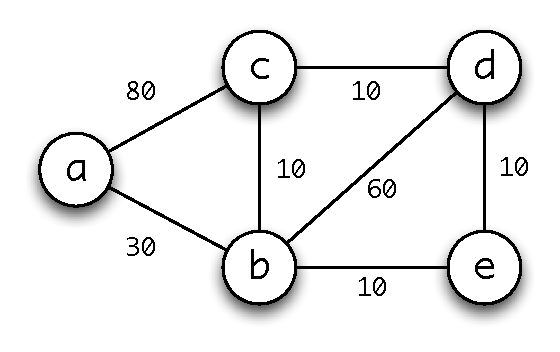
\epsfig{file=eps/flight-costs.eps,width=0.45\columnwidth}
\caption{Flight Map and Cost Between 5 Cities}
\label{fig:flight}
\end{figure}

\begin{figure}[tb]
\begin{lstlisting}[label=lst:tsell,caption=Ticket Seller's Agent. \texttt{[...]} denotes a list while \texttt{X[$i$]} is the $i$-th element of list \texttt{X}. \texttt{rand($m$)} returns a random integer between $0$ and $m$ (inclusive). \texttt{X.Y} denotes the concatenation of symbols so that \texttt{u.v} evaluates to \texttt{uv}.]
Ts = [[a,b,30],[a,c,80],[b,c,10],
      [b,d,60],[b,e,10],[c,d,10],[d,e,10]]
loop
  T = Ts[rand(6)]
  if rand(1) = 0
    |$\Out$|(ticket, T[0].T[1], T[2])
  else
    |$\Out$|(ticket, T[1].T[0], T[2])
|$\exit$|
\end{lstlisting}
\begin{lstlisting}[label=lst:tbuy,caption={Ticket Buyer's Agent. Both {\tt fly()} and {\tt try()} are defined using pattern matching on parameters. \texttt{[N:Ns]} denotes a list which has \texttt{N} as its head and \texttt{Ns} as its tail. Underscore (\texttt{\_}) matches anything in the context of pattern matching.}]
fly(X, X, Cash, V): arrived
fly(X, Y, Cash, V): Ns = unvisited_neighbors(X, V)
                    try(X, Ns, Y, Cash, V)

try(X, [N],    Y, Cash, V): buy(X, N, Y, Cash, V)
try(X, [N:Ns], Y, Cash, V): (buy(X, N, Y, Cash, V)
                            |$\oplus$|try(X, Ns, Y, Cash, V))
                            |$\cm$|

buy(X, N, Y, Cash, V):
  |$\In$|(ticket, X.N, |$\lambda x.x\le\texttt{Cash}$|) = (_, _, Cost)
  fly(N, Y, Cash - Cost, [N:V])

fly(a, e, 100, [a])
|$\exit$|
\end{lstlisting}
\vspace*{-5mm}
\end{figure}

\subsubsection*{Stock Trading (ST)}

In this example, we set up a mini stock market which follows the prices in the public exchange 
but is not openly available to the public. 
Traders can join the market at any time but their trades will not affect the public market.
Markets like this do exist in real life in the form of 
``Dark Pools''\cite{degryse2008shedding}  
which offers anonymous and private investors to
trade away from the public exachanges.

Our market starts with $N$ stocks, each has a fixed amount of shares dedicated for this market.
In general, each trader has a fixed amount of money in the beginning, 
and can buy (or sell) stocks from (or to) the market according to the public prices.
% Each trader also has a high watermark and a low watermark of cash.
% When the cash value is less than the low watermark (or greater than the high watermark), 
% the trader will keep selling (or buying) stocks in order to increase (or decrease) the cash value. 
% This strategy comes from real-world strategies where people want to control the risk.
% Different watermarks lead to different behaviors, and for this example, 
% the traders speculate to be either conservative or aggressive.
Listing \ref{lst:trader} shows the trader's agent program. 
Each trader trades several rounds until his cash value reaches the goal. 
For each round, the trader randomly picks a stock {\tt X}, buys it as much as possible, 
and waits for the price of {\tt X} to change. 
$\alpha$ is a value between 0 and 1 which indicates the profit/loss margin percentage. 
For example, if a trader buys {\tt X} at a price of {\tt P}, 
he sells it at a price of either higher than $(1+\alpha)\times{\tt P}$ (to profit)
or lower than $(1-\alpha)\times{\tt P}$ (to prevent further loss). 
Different $\alpha$ values lead to different trading behaviors, and for this example,
the traders speculate to be either 
conservative (smaller $\alpha$) or aggressive (larger $\alpha$).
Note that there is no atomicity guarantee between checking the price of a stock 
and actually buying it, which is also the behavior of a real market.
Also an intention to buy can be partially filled by the stock-serving agent
(see Listing \ref{lst:stock}).
The stock-serving agent also waits for price updating (i.e. {\tt (update, ...)})
from the public exchange in a realtime fashion. 

\begin{figure}[tb]
\begin{lstlisting}[label=lst:trader,caption={Trader's Agent. Numbers are irrelevant and just for illustration purposes.}]
Me     = unique_account_name
Stocks = [...]  // a list of stock names
Start  = 5000   // start with cash of $5000
Goal   = 5500   // the goal is to end up with $5500

trade(Cash, |$\alpha$|):
  X = Stocks[rand(N-1)]

  |$\Rd$|(price, X, _) = (_, _, P1)
  Q1 = |$\lfloor$|Cash / P1|$\rfloor$|
  |$\Out$|(buy, X, Q1, Me)
  |$\In$|(ack, Me, _, _) = (_, _, P2, Q2)
  C1 = Cash - P2 * Q2

  |$\Rd$|(price, X, |$\lambda x.x\ge(1+\alpha)\times{\tt P2}\lor x\le(1-\alpha)\times{\tt P2}$|)
  |$\Out$|(sell, X, Q2, Me)
  |$\In$|(ack, Me, _) = (_, _, P3)
  C2 = C1 + P3 * Q2

  if C2 < Goal
    trade(C2, |$\alpha$|)
  else
    |$\cm$|

trade(Start, 0.01) |$\oplus$| trade(Start, 0.05)
|$\exit$|
\end{lstlisting}
\begin{lstlisting}[label=lst:stock,caption=Stock-serving Agent. \texttt{P} is the current price of the stock while \texttt{Q} is the quantity of stocks available for sale.]
Me = unique_stock_name

serve(P, Q):
  case |$\In$|(_, Me, _, _)
    (update, _, NewPrc, _): |$\In$|(price, Me, _)
                            |$\Out$|(price, Me, NewPrc)
                            serve(NewPrc, Q)

    (buy, _, Q1, X): Q2 = min(Q1, Q)
                     |$\Out$|(ack, X, P, Q2)
                     serve(P, Q - Q2)
    
    (sell, _, Q2, X): |$\Out$|(ack, X, P)
                      serve(P, Q + Q2)

|$\Out$|(price, Me, Start_Price)
serve(Start_Price, Start_Quantity)
\end{lstlisting}
\vspace*{-6mm}
\end{figure}

\subsubsection*{Dining Philosophers (DP)}

% \begin{figure}[tb]
% \centering
% 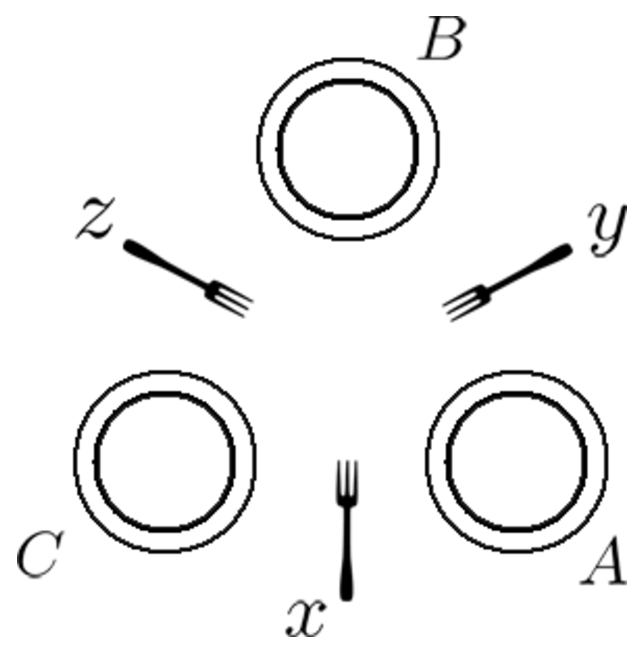
\epsfig{file=eps/dining.eps,width=0.3\columnwidth}
% \caption{Three Dining Philosophers Problem.
% $A,B,C$ are philosophers while $x,y,z$ are forks.}
% \label{fig:dining}
% \end{figure}

% \RY{can delete the figure. Listing 9 can be joined horizontally rather
% than vertically as now}

Consider the well-known ``Dining Philosophers Problem''
\cite{Dijkstra2002:Hierarchical} - there are three
philosophers $A$, $B$ and $C$, sitting around a dining table,
with three forks $x$, $y$ and $z$ between them.
This classic concurrency problem
shows that deadlock happens with certain sequences of acquiring the forks,
e.g., $A$ acquires $x$, $B$ acquires $y$ and then
$C$ acquires $z$. 
The classic solution to this problem is using a synchronization mechanism 
such as a counting semaphore, imposing a partial order on acquiring the forks, 
or requiring one philosopher to be asymmetric.
However, such kind of solution requires additional constraints to the problem. 
%
In this example, the speculation framework offers an alternative
solution which is purely based on the definition of the problem.
We extend the problem to $N$ dining philosophers 
sitting around a table with $N$ forks.
For simplicity, each philosopher has a unique index ranging from $0$ to $N-1$. 
Listing \ref{lst:dpinit} shows the initialization of data stores 
for dining philosophers.
Listing \ref{lst:dp} shows the agent program for dining philosophers.
\texttt{my\_index()} returns the index of the current philosopher.

\begin{figure}[tb]
\begin{lstlisting}[label=lst:dpinit,caption=Dining Philosophers (initialization)]
for I = 0 to N-1
  |$\Out$|(fork,I)
|$\exit$|
\end{lstlisting}
\begin{lstlisting}[label=lst:dp,caption={Dining Philosophers. \texttt{\%} denotes the modulo operation. {\tt ;} separates multiple statements in one line. $\Out$ is non-blocking in the tuple space data model, so we don't need choices for putting back forks.}]
L = my_index(); R = (L+1) % N
(|$\In$|(fork,L); |$\In$|(fork,R)) |$\oplus$| (|$\In$|(fork,R); |$\In$|(fork,L))
|$\cm$|
|$\Out$|(fork,L); |$\Out$|(fork,R)
|$\exit$|
\end{lstlisting}
\shrink
\shrink
\end{figure}

By using such kind of speculation, it can be guaranteed that 
there is always one world where nobody deadlocks. 
For example, assume $N=3$, the combination of the choices from three philosophers 
theoretically creates eight worlds as in Figure \ref{fig:diningrun} 
(though in practice some of the worlds may never be there due to pruning).

\begin{figure}
\centering\small
\Tree[.$\oplus_A$
    [.$\oplus_{B_1}$
        [.$\oplus_{C_1}$
            {$A\compact:-x$ \\ $\quad-y$ \\ $B\compact:-y$ \\ $\quad-z$ \\ $C\compact:-z$ \\ $\quad-x$ \\ $(w_1)$}
            {\bk$A\compact:-x$ \\ \bk$\quad-y$ \\ \bk$B\compact:-y$ \\ \bk$\quad-z$ \\ \bk$C\compact:-x$ \\ \bk$\quad-z$ \\ $(w_2)$}
        ][.$\oplus_{C_2}$
            {$A\compact:-x$ \\ $\quad-y$ \\ $B\compact:-z$ \\ $\quad-y$ \\ $C\compact:-z$ \\ $\quad-x$ \\ $(w_3)$}
            {\bk$A\compact:-x$ \\ \bk$\quad-y$ \\ \bk$B\compact:-z$ \\ \bk$\quad-y$ \\ \bk$C\compact:-x$ \\ \bk$\quad-z$ \\ $(w_4)$}
        ]
    ][.$\oplus_{C_3}$
        [.$\oplus_{B_2}$
            {$A\compact:-y$ \\ $\quad-x$ \\ $B\compact:-y$ \\ $\quad-z$ \\ $C\compact:-z$ \\ $\quad-x$ \\ $(w_5)$}
            {\bk$A\compact:-y$ \\ \bk$\quad-x$ \\ \bk$B\compact:-z$ \\ \bk$\quad-y$ \\ \bk$C\compact:-z$ \\ \bk$\quad-x$ \\ $(w_6)$}
        ][.$\oplus_{B_3}$
            {$A\compact:-y$ \\ $\quad-x$ \\ $B\compact:-y$ \\ $\quad-z$ \\ $C\compact:-x$ \\ $\quad-z$ \\ $(w_7)$}
            {\bk$A\compact:-y$ \\ \bk$\quad-x$ \\ \bk$B\compact:-z$ \\ \bk$\quad-y$ \\ \bk$C\compact:-x$ \\ \bk$\quad-z$ \\ $(w_8)$}
        ]
    ]
]
\caption{Three Dining Philosophers Problem (tree of choices). Minus sign ($-$) denotes taking the fork. Deadlock only happens in $w_1$ and $w_8$.}
\label{fig:diningrun}
\shrink
\end{figure}

There are many practical algorithms and applications (e.g., 2-phase locking)
that are special cases or extensions of the Dining Philosopher Problem (DPP). 
So we generalize DPP as follows.
\begin{definition}[Generalized Dining Philosopher Problem]
Given a set of resources $R$ which are available at the beginning, 
$n$ agents each interested in a subset of resources 
$R_i\subseteq R (1\le i\le n)$, and each agent is a two-phase process:
  \begin{enumerate}
    \item In the \emph{acquisition phase} the agent consumes every resource $r\in R_i$ in any order;
    \item In the \emph{release phase} the agent puts back every resource $r\in R_i$ in any order.
  \end{enumerate}
  $R_i$'s may overlap so the scheduler may produce a schedule which can cause deadlock 
among the agents.
\end{definition}

\begin{theorem} Generalized Dining Philosopher Problems do not deadlock 
using speculative nondeterminism.
\end{theorem}
\begin{proof}[Proof sketch]
% first show there is always a solution
First, we construct a combination of choices which will never deadlock. 
Fix an ordering of the elements in $R$, for example $r_1,r_2,\dots,r_m$ where $m=|R|$. 
For any agent $i$, it consumes $R_i$ in this fixed order. 
Then there will be races instead of deadlocks because there will not be the 
case that agent $i$ consumes $r_x$ and waits for $r_y$, and agent $j$ consumes
$r_y$ and waits for $r_x$ ($x<y$ and $y<x$ cannot be true at the same time). 
% then show the solution will not be pruned
Then it can be shown this combination will not be pruned by commits in an 
eventually blocking world due to the commit semantics described in rule \ref{rule:cm}. 
\end{proof}


\begin{figure}[ht!]
\centering
% TODO: use a tabular{cr} to format better
\flushright\fbox{Entrance transition: $T\|a\Longrightarrow T'$}
\[
  \tag{\sc Entrance1}\label{rule:entrance1}
  \langle A,D,S\rangle \| a \Longrightarrow \langle A+[a],D,S\rangle
\]
\[
  \tag{\sc Entrance2}\label{rule:entrance2}
  T_1\oplus_k T_2 \| a \Longrightarrow (T_1 \| a)\oplus_k (T_2 \| a)
\]
\flushright\fbox{Tree transition: $T\To T'$}
\[
  \tag{\sc Swap}\label{rule:swap}
  T_1\oplus_k T_2 \To T_2\oplus_k T_1
\]
\[
  \tag{\sc DataOp}\label{rule:dataop}
  \frac
  {A[k]=d.e:f \qquad D\vdash d \qquad \langle t,D'\rangle=\psi(d,D)}
  {\langle A,D,S\rangle \To \langle A[k\mapsto t.e:f], D', S\rangle}
\]
\[
  \tag{\sc Choice}\label{rule:choice}
  \frac
  {\begin{matrix}
    A[k]=(e_1\oplus e_2).e:f \\
    T_1=\langle A[k\mapsto e_1.e:f],D,S\rangle \\
    T_2=\langle A[k\mapsto e_2.e:f],D,S\rangle
   \end{matrix}}
  {\langle A,D,S\rangle \To T_1\oplus_k T_2}
\]
\[
  \tag{\sc Cm}\label{rule:cm}
  \frac
  {A[k]=\cm.e:f}
  {\langle A,D,S\rangle\oplus_k T \To \langle A[k\mapsto e:f],D,S\rangle}
\]
\[
  \tag{\sc Cu}\label{rule:cu}
  \frac
  {A[k]=\cu.e:f}
  {\langle A,D,S\rangle\oplus_k T \To T}
\]
\[
  \tag{\sc Exit1}\label{rule:exit1}
  \frac
  {A[k]=\exit.e :f \qquad s=\langle k,f(D)\rangle}
  {\langle A,D,S\rangle \To \langle A[k\mapsto\exiting],D,S\cup\{s\}\rangle}
\]
\[
  \tag{\sc Exit2}\label{rule:exit2}
  \frac
  {\begin{matrix}
    \forall w\in leaves(T): exiting(w,k) \land v = exitv(w,k)
   \end{matrix}}
  {T \To exit(T,k)}
\]
\[
  \tag{\sc Collapse}\label{rule:collapse}
  \frac
  {\begin{matrix}
    w \in leaves(T) \\
    \forall k: exiting(w,k) \lor exited(w,k)
   \end{matrix}}
  {T \To w}
\]
\flushright\fbox{Local computation transition: $e\computes e'$}
%\begin{align*}
\[
\begin{array}{llll}
  e &\computes op.e' \hspace*{5mm} &
  e &\computes \epsilon \\
  t.e &\computes e' &
  e_1.e_2 &\computes e_1'.e_2 \\
\end{array}
\]
%%  \epsilon.e &\computes e
%\end{align*}
\flushright\fbox{Helper functions}
\begin{gather*}
  \frac
  {T = T_1\oplus_k T_2}
  {leaves(T) = leaves(T_1)\uplus leaves(T_2)} \\
  leaves(w) = \lbb w\rbb \\
  \frac
  {w=\langle A,D,S\rangle \qquad \langle k,v\rangle\in S}
  {exitv(w,k) = v} \\
  \frac
  {w=\langle A,D,S\rangle}
  {exiting(w,k) = (A[k]=\exiting)} \\
  \frac
  {w=\langle A,D,S\rangle}
  {exited(w,k) = (A[k]=\exited)} \\
  \frac
  {T = T_1\oplus_i T_2}
  {exit(T,k) = exit(T_1,k)\oplus_i exit(T_2,k)} \\
  \frac
  {w=\langle A,D,S\rangle}
  {exit(w,k) = \langle A[k\mapsto\exited],D,S\rangle}
\end{gather*}
\caption{Semantics of the Speculation Language.
$[\dots]$ denotes a list,
$A[k]$ is the $k$-th element in list $A$, and
$A[k\mapsto x]$ denotes the updating of the $k$-th element to $x$.}
\label{fig:semantics}
\end{figure}

\subsection{Semantics}\label{sec:semantics}

The semantics of the speculation language is 
given in \figref{fig:semantics}. 

\paragraph*{Entrance}
New agents can dynamically enter the system at any time.
\ref{rule:entrance1} and \ref{rule:entrance2} the addition of
a new agent $a$ to the system (denoted $\|$). The Plus sign ($+$) 
denotes list concatenation. The whole tree is recursively traversed and $a$ is appended to the agent list in every world. 

\paragraph*{Choice Symmetry}
\ref{rule:swap} shows that the two branches of an interior node in the tree are treated equally.

\paragraph*{Data Operation}
An agent wants to execute operation $d$ on the data store $D$
(see \ref{rule:dataop}).
This transition first has to meet condition $D\vdash d$. 
The effect of $d$ on data store $D$ is defined by
the transition function $\psi$ in the data model and it only
affects the current world having store $D$
without affecting other worlds in the tree.
The result of $d$ is denoted is $t$ and provided to the remaining local 
computation $e$ as a parameter (denoted by the special syntax $t.e$). 
$t.e$ is not processed by the speculation framework, but 
activates the local computation $e$ and will eventually transform to another 
local computation $e'$ (i.e. $t.e\computes e'$). 

\paragraph*{Local Computation}
The local computation transition is simply a placeholder for
the semantics of the actual computation in the host language.
As that is orthogonal to our semantics, the details are left
unspecified. There is one special operation, $t.e$, which applies
the result of a data operation $t$ to some local computation $e$.
For example, it might be to store $t$ in a variable in the host language.
% \KZ{The following may need to be changed:\\
% We shall omit the details of the language in which 
% local computations are expressed and just assume that
% there exist a local computation transition $\computes$.
% From the perspective of the speculation framework, 
% the only thing that matters is the operation $op$ 
% produced by a local computation. 
% As shown in \figref{fig:semantics}, 
% a local computation $e$ transforms to $op.e'$ to 
% execute $op$ under the framework, or to $\epsilon$ to 
% finish execution. 
% After a data operation which reads something from the data store,
% a data item $t$ in the store is returned to the local computation $e$, 
% and further transforms to a new local computation $e'$, which is 
% $e$ parameterized by $t$. 
% $e_1.e_2$ denotes sequential execution of $e_1$ and $e_2$. 
% After $e_1$ transforms to $\epsilon$, $e_2$ starts execution 
% ($\epsilon.e\computes e$).
% }

\paragraph*{Choice and Commit}
Speculative nondeterminism provides for the creation and subsequent
pruning of choices. 
\ref{rule:choice} fires if an agent is reduced to a choice $(e_1\oplus e_2).e$, 
and it consumes the choice construct in the agent to split the current world into two
(i.e. $T_1$ and $T_2$). 
Section \ref{sec:commit} discusses further the ramifications of commit,
here, we start with first describing what the commit rules do.
When the $k$-th agent executes $\cm$ in a leaf world of the tree structure, 
as shown in rule \ref{rule:cm}, the other side of the choice (i.e. $T$) is pruned
only if the current choice node is $\oplus_k$. 
Similarly, $\cu$ is used where the agent wants to explicitly gives up the current choice branch,
so the current side of the choice is pruned, 
as shown in rule \ref{rule:cu}. 
$\cm$ and $\cu$ are symmetric and both of them are {\em commit} operators.
Commit of the $k$-th agent can only be executed in a world with $\oplus_k$ as its parent,
and it is blocking when the parent node is not $\oplus_k$.
%which makes the commit more localized and less aggressive. 
% This form of commit semantics is therefore known as {\em localized commit}.
%With this commit semantics, it only affects a small fraction of the whole tree. 
%Also it is possible to make pruning decisions locally, which makes it efficient. 

\paragraph*{Exit}
In general, a single agent will have many versions of itself executing
in all the multiple virtual worlds.
Thus, if it were simply to exit from all the worlds on the first
$\exit$ operation, this could lead to some form of data inconsistency.
We deal with this using the exit function $f$ specified by each agent which
allows an agent-specific consistency condition to be used.
Note that different agents may be interested in different aspects of the data store. 
When an agent exits, all the worlds should look the same from the perspective of that agent. 
However, another agent may not consider the worlds to be the 
same since it can have a different exit function. 
This also means that an agent properly exiting is only achieved when
the consistency requirement is obtained.

Rule \ref{rule:exit1} and \ref{rule:exit2} shows the exit semantics. 
\ref{rule:exit1} shows the case when an {\em instance} 
of the $k$-th agent reaches $\exit$ in a world. 
In this case, the exit function $f$ is applied to the current data store $D$ and a {\em snapshot} 
is created and added to $S$. 
 
The exit function $f$ takes a data store as input, and returns an integer as the evaluated result. 
The data store is just the one associated with the current world. 
According to the data store, the exit function is expected to produce an integer 
which can be a 0/1 indicator, a heuristic value, or an encoding of more complicated mathematical objects. 
For example, in the simplest case, $f(d)\equiv 1$ allows the agent to exit without any condition 
as long as it completes execution of all the operations in the program. 
The ability to return an integer provides more flexibility and enables 
complex exiting logic to be embedded in this exit function.

While taking a snapshot, 
the agent in that world switches to a special state $\exiting$.
\ref{rule:exit2} checks all the worlds in the tree. Only if (i) the $k$-th agent has 
switched to $\exiting$ state in all the worlds, and (ii) the exit value $v$ of the $k$-th agent 
is {\em identical} across all the worlds, 
then the $k$-th agent can exit from the worlds at the same time. 
For \ref{rule:exit2}, the exit value $v$, which can be thought of as the return value from
the speculative computation, will be eventually provided to 
a local computation $\tilde e$
which is completely outside the system of virtual worlds, 
and has no more speculation and data store operations. 
The idea of this type of consistent exit across all worlds is analogous
algebraic factorization, i.e.
$ab + ac = a(b+c)$.

\paragraph*{Collapse}
Note that commit is optional in an agent program, so the agents can 
let the tree expand without pruning, and finally leave the tree 
without reducing to one world. 
Therefore some agents may never exit due to the inconsistency of some worlds, 
even if all the agents have finished execution.
\ref{rule:collapse} handles this case 
to let these agents exit as well as to reclaim system resources. 
The system could employ a global collapse rule to pick any world where 
all agents have completed execution and reduce the tree to one world.
For \ref{rule:collapse}, the exit value for every agent $k$ is also returned in this way.
$\tilde e$ can make use of the exit value to extract what the agent concerns. 
%\KZ{Need to say exit is implicit if it's not added to the program?}

\paragraph*{Helper Functions}
We also define a set of helper functions to simplify the semantics. 
\begin{description}
\item[$leaves(T)$] returns a multi-set of the leaf worlds in tree $T$. 
\item[$exitv(w,k)$] retrieves the exit value, i.e. the evaluation result of the exit function, of the $k$-th agent in world $w$.
\item[$exiting(w,k)$] is a predicate indicating whether the $k$-th agent in world $w$ is in the special state of $\exiting$.
\item[$exited(w,k)$] is a predicate indicating whether the $k$-th agent in world $w$ is in the special state of $\exited$.
\item[$exit(T,k)$] switches the $k$-th agent in all the worlds in $T$ to the special state of $\exited$.
\end{description}

\subsection{More on Commit}\label{sec:commit}
Commit is a special and important operation in speculative nondeterminism because:
(i) it gives the agent the power to specify preferences among different choices,
e.g., in Listing \ref{lst:intro-commit-sleep}; 
(ii) it prunes some of the virtual worlds to make it easier for agents to exit
because the fewer remaining worlds means easier consistency checks,
and thus it improves the responsiveness and overall throughput of the system;
(iii) by pruning worlds, it also reclaims precious system resources such as
memory and CPU cycles, which is critical to the viability of the multi-world 
speculation , even though the naive combinatorial problem space is exponential and
prohibitive.

However, it is also important to understand that whenever commit is used and
pruning is done, potential solutions can be pruned away, and deadlock or blocking
may arise as a result. So from the system point of view, we design a commit
semantics that is {\em localized} and less aggressive because the scope of the pruning
is restricted to be of height 1 only and affects only a small fraction of
the whole tree (see Rule \ref{rule:cm}). This commit semantics is also
more efficient because pruning decisions are made locally. There are of course
other possible commit semantics \cite{JaffarYZ07} which are more eager in pruning. 
For example, one type of commit requires agent $T$ to commit in all left or right
subtree rooted at $\oplus_T$. These are either too aggressive and lose 
too many solutions or require coordination
among various worlds which is more costly to execute in practice.

From the programmer's point of view, she should use commit with care, knowing that
without commit, the multi-world space grows very quickly and the program probably
cannot scale, but with commit, the program could potentially lose valuable solution.
It makes more sense to put commit later rather than early in the choice. 
If one must put a commit in the middle of a sequence of operations like
$op_1.op_2.\cm.op_3.op_4$, she should ensure that the remaining operations
after $\cm$, i.e., $op_3$ and $op_4$, are not likely to block, 
e.g., when they are local computations.

%The commit semantics described in Section \ref{sec:semantics} 
%is called {\em localized commit} as it restricts
%the scope of pruning to be of height 1 only.  
%%$\cm$ by agent $X$ cannot
%%prune until the direct parent of the committed world is $\oplus_X$.
%%$\cu$ kills the current world immediately without coordination with other worlds.
%Besides localized commit, there is a number of other possible commit
%semantics \cite{JaffarYZ07}.
%They differ in their eagerness to prune the worlds.
%They are ordered roughly from the most eager to the most conservative:
%{\em absolutely eager commit}, {\em eager commit}, {\em coordinated commit}, 
%{\em late commit} and {\em no commit}. 
%



\section{Framework}
%\BF{workflow figure to show the framework}
%\begin{multicols}{2}
%\begin{figure*}
%\centering
%\includegraphics[width=2\columnwidth]{sysoverviewgrapheps.eps}
%\caption{Framework wrokflow} \label{fig:workflow}
%\end{figure*}
%\end{multicols}
%\KZ{In the framework, say ``Output Parse'' instead of ``Output File.''}
The general architecture of the our parser is shown in \figref{fig:workflow}
and is divided into training phase and parsing phase.
%We take training treebank as input, which carries the
%essential information (we only use FORM and POSTAG) and
%gold dependency parses.

\begin{figure}[th]
\centering
\epsfig{file=sysoverviewgrapheps.eps, width=\columnwidth}
\caption{Sequence Based Parser Framework}
\label{fig:workflow}
\end{figure}

{\bf Training:} The preprocessing step generates oracle sequences
from the gold standard parse trees. Only the word forms and the POS tags 
in these parse trees are used. Here, we assume that a child node is
easier to process than its parent node and it is supposed to be attached
before its parent. \footnote{By this rule, multiple gold sequences
can be generated from one dependency tree. In this paper, when a parent node
has multiple children, we generate the sequence by a left-to-right order.}
%\KZ{Which one do we use or do we use all of them?}
%\footnote{
%For example, a bottom-up, breadth-first traversal of the gold parse tree or oracle transition
%process order from Malt Parser are both gold sequences.}
%and further discussion is deferred to Section 4.
%\TJ{maybe they will ask which one is the best; needs some explanations here}
We then train respectively a graph-based head mapper (a.k.a. decoder)
from the gold sequences and the gold parses, and a sequence predictor
from the gold sequences.

{\bf Parsing:} Given an input sentence, the sequence predictor
outputs a feasible decoding sequence, which is a permutation of
the words in the input. For each word in this sequence,
the head mapper returns its best head word according to a scoring function
while employing a cycle detection mechanism.
The process continues until all words in the sentence have found their
heads.
%(except manually introduce ROOT node in dependency parsing).
%For a sentence with $N$ words, the final result consists of ($N+1$) nodes
%and constructed $N$ arcs.
The procedure guarantees to produce a tree structure eventually.
\cut{
We implemented a simple version of this framework,
%and released the source code as well as the evaluation data\footnote{\urlstyle{same}\url{https://github.com/littlebeanfang/BeanParser}}.
%To reproduce the experiments refered in this paper, all our data and related commands are offered in the compressed file.
%\BF{add the data download source}
%\KZ{Besides the open-source system, create an online demo using default model
%and allow users to type in
%a sentence to have it parsed.}
and built an online demo\footnote{\urlstyle{same}\url{http://202.120.38.146/BeanParser}} to show parses of eight languages with the model
trained in our experiment.}

In the current implementation, we generate the decoding sequence by
{\em stackproj} algorithm~\cite{nivre2009non} in
malt parser and scorer-based greedy head mapper.
%\KZ{Consider rephrase this sentence.
%What does graph-based head mapper have to do with sequence?}
%The training and testing data are both in
%CoNLL format~\footnote{http://ilk.uvt.nl/conll/}.


\section{Experiments}
\label{sec:experiments}
In this section, we conduct
extensive experiments on slogan generation 
to evaluate the performance
of the proposed model SALE.
We introduce the dataset, 
the competing models and parameter settings,
as well as the evaluation metrics.
We also demonstrate the experimental results in a series of evaluations
and perform further analyses on the effectiveness of our approach
in generating accurate, fluent, informative and attractive slogans.

\subsection{Dataset}
\label{sec:dataset}
We first introduce the text corpora we create
for slogan generation task in e-commerce.
Then we describe the evaluation dataset we used in
our following experiments.
The datasets are released at \url{https://202.120.38.146/slogan/}.

\subsubsection{Dataset for Slogan Generation}
\label{sec:corpora}
%In this section, we describe the experimental setup,
%especially the hyper-parameter configurations of 
%the Seq2Seq framework we used in following experiments. 
%We also detail dataset used in our experiments.
Slogan generation in E-commerce is a relative new problem.
Thus, there is a lack of dataset for this task.
We created a new dataset, containing 
the basic information of the topics attending to potential focuses or selling-points,
including the topic and its item preference, as well as the slogan.
The data are collected from Taobao, a large-scale website for e-commerce in China.

We use the pattern of ``\emph{PV} + \emph{CG}" 
to construct topics from frequent phrases mining from largely amount
of query logs and product titles.
The product titles are composed by the sellers and content producers on the
website.
We construct multiple item preferences for each topic by sampling items from 
secondary categories as well as human intervention to 
make the items with an item preference concentrate more on a specific focus 
or selling-point.
Thus, in each instance, a topic is annotated with an item preference semi-automatically
by leveraging the category ontology introduced in \secref{sec:introduction}.
Then, we recruit experts to write a slogan for each data instance.
Overall, the dataset contains 857 topics and 
in total 3,555 $(x, p, y)$ instances after preprocessing.

We use four splits named (train/dev/LMdev/test) in our experiments.
Note that, the LMdev split is for 
hyper-parameter $\beta$ tuning (see \secref{sec:shallow_fusion} in details).
The splits are randomly divided based on topics 
proportionally by 90\%, 5\%, 1.5\% and 3.5\%.
Thus each split of (train/dev/LMdev/test) includes 771, 43, 13, 30 topics separately,
and correspond to 3132 training instances, 231 development instances, 
50 LM development instances, as well as 142 test instances.

%For the evaluation dataset, 
\subsubsection{Evaluation Dataset}
\label{sec:eval_dataset}
We perform algorithm evaluation and human evaluation
in our experiments (see \secref{sec:metrics} in details).
Thus we provide two evaluation datasets separately for each.
We directly use all the 142 instances of test split in \secref{sec:corpora},
referred as FULLtest,
for the algorithm evaluation which are based on automatic scoring systems,
such as BLEU.
Besides, we randomly sample 50 instances from the test split
to form a small evaluation dataset for human evaluation,
referred as HUMtest.


\subsection{Compared Methods}
\label{sec:compared}
In this section, we introduce the baseline and choices for 
our model components, as well as the parameter settings
used in those models.

\subsubsection{Baselines and SALE}
\label{sec:baselines}
According to the problem statement (in \secref{sec:problem})
and the proposed item preference fusion methods (in \secref{sec:preference}),
the models for comparison backed by Seq2Seq framework are mainly one-way input models and two-way input models.

One-way input models (prefixed by \emph{One}) takes in one-way input as the source sequence,
and the slogan as its target sequence, without considering 
semantics enhancement or incorporating pretrained language model.
There are three one-way input baselines with different inputs.
\textbf{One-T} (\textbf{t}opic) model
takes the topic itself as its source sequence,
while \textbf{One-P} (item \textbf{p}reference) model takes
the titles of items as its source sequence.
Then, 
%while 
\textbf{One-CAT} (con\textbf{cat}nating) model 
concatenates the topic and its item preference with special token \emph{SEP}
as a separator, and takes the sequence of concatenation as its source sequence.

The two-way input models (prefixed by \emph{Two})
are designed to treat topics and item preferences heterogeneously.
We propose two kinds of two-way input models
based on different heterogeneous inputs fusion methods 
(see details in~\secref{sec:preference}).
%we propose two fusion methods in \secref{sec:preference}
%to combine the heterogeneous inputs.
\textbf{Two-BiAttn} (\textbf{bi}directional \textbf{att}ending) model use the two-way bidirectional attending
to combine the representations of topics and that of item preferences.
\textbf{Two-CAT} (con\textbf{cat}nating) model use two-way concatenating strategy 
to fuse the heterogeneous outputs of encoders.

For \textbf{SALE}, 
we incorporate the semantics enhancement module
(in \secref{sec:semantics}) to enrich
the deep contextualized representations
backed by Two-CAT baseline.
\textbf{SALE+PLM} integrates
%On the basis of SALE, 
%we integrate
pre-trained language model (PLM) 
into SALE at inference time in order to improve
the generalization and robustness of the model.
%Specially, SALE identifies the \emph{is-a} relations
%among heterogeneous inputs and
%increase the semantic capacity of the model for better contextualized representations
%knowledge-aware module

\subsubsection{Parameter Settings}
We use an architecture of 8 stacked convolutional layers 
for both the topic encoder and the item preference encoder
as well as the decoder parts with kernel width as 3.
To enable deep convolutional networks, 
we add residual connections~\cite{he2016deep} from the input of each convolution
to the output of the layer as well.
For each convolutional layer, we set the hidden vector size as 512
and the embedding size as 256.
To alleviate the overfitting problem, we add the dropout ($p=0.2$)
layer~\cite{srivastava2014dropout} for all convolutional layers and fully connected layers.

To optimize the proposed models,
we use Nesterov's accelerated gradient method
~\cite{sutskever2013importance} with gradient clipping 0.1
~\cite{pascanu2013difficulty},
momentum 0.99, and 
learning rate 0.2.
We terminate the training process when the learning rate drops 
below 10e-5.
We set beam size as 5 for the beam search algorithm
in the testing step.
The hyper-parameter $\beta$ of SALE-PLM (in ~\eqnref{eq:shallow_fusion})
was selected to maximize the generation performance
on the LMdev split by grid search, from the range 1e-4 and 0.1.


\subsection{Evaluation Metrics}
\label{sec:metrics}
We perform both algorithm evaluation and human evaluation
in our experiments.
Specially, we evaluate our model on generation quality which includes
the automatic scoring metrics such as
BLEU and lexical diversity,
as well as a number of human-evaluation metrics.

\paragraph{BLEU}
The BLEU algorithm~\cite{papineni2002bleu} compares consecutive phrases of the 
generated slogan with the consecutive phrases it finds
in the reference slogan, and counts the number of matches, in a weighted fashion.
A higher BLEU score indicates a higher degree of similarity with the reference
slogan.
We compare all competing models on test split in terms of the BLEU score as a sanity check.
We also use BLEU score as the standard metric to finetune
hyper-parameter $\beta$ in SALE+PLM model.

\paragraph{Lexical Diversity}
A common problem in automatic text generation is that the system tends to generate safe
answers with enough diversity~\cite{li2016deep}.
A low diversity score often means generated contents are general and vague, 
while higher diversity means the generated contents are more informative and 
interesting.
Following~\cite{ChenLZYZ019}, we calculate the number of distinct n-grams produced on the test split
as the measurement of the diversity of generated descriptions.

\paragraph{Human-evaluation Metrics}
Automatic scoring metrics including BLEU score and lexical diversity are competitive and inexpensive to operate.
However, they do not consider
other important aspects such as intelligibility and grammatical correctness (or fluency) of slogan.
We use several human-evaluation metrics
to evaluate competing models on various perspectives.
\begin{itemize}
	\item \textbf{Overall quality} is designed to measure the
	overall generation quality of model.
	\item \textbf{Relevancy} is used to measure the content relevancy of generated slogan to the given topic and items.
	\item \textbf{Fluency} focus on the intelligibility and grammatical correctness of generated slogan.
	\item \textbf{Interestingness} takes personification and attractiveness into account.
\end{itemize}


\subsection{Performance Comparisons and Analysis}
\label{sec:results}


In this section, we conduct an analysis of our proposed model
to evaluate the contribution of item preference fusion module and
semantics enhancement module as well as the integration of 
pre-trained language model.

We evaluate competing models on FULLtest and HUMtest 
as we described in \secref{sec:eval_dataset}.
The comparison results of slogan generation are shown in 
\tabref{tab:auto_eval} and \tabref{tab:human_eval}.
For human evaluation, we recruit three experts as annotators 
and ask them to give scores on each aspect of generated slogan, 
range from 1 to 5,
then average the scores of each aspect on HUMtest as 
human evaluation results.


\begin{table*}[th]
	%	\small
	\centering
	\caption{Slogan generation results comparison with baseline methods using FULLtest.}
	\label{tab:auto_eval}
	\begin{tabular}{lcccc}
		\hline
		Model %& Overall quality 
		& BLEU &  Diversity (n=2) ($\times 10^2$ )& Diversity (n=3) ($\times 10^2$ ) & Diversity (n=4) ($\times 10^2$ ) \\
		\hline
		One-T %&  3.30  
		&  28.34 &  2.25   &  2.45  &  2.37 \\
		One-P %&  3.86  
		&  41.11 &   4.74 &    5.99 & 6.33 \\
		One-CAT  % & 3.82  
		& 38.86  &  3.86 &  4.77  & 4.94 \\
		Two-BiAttn  % & 3.86  
		& 36.99  &  4.82 &  5.87  &  6.03   \\
		Two-CAT % & 3.95
		& 40.59  &  4.89 &  5.99  &  6.22 \\
		\hline\hline
		SALE % & \textbf{4.16}  
		& 42.31  & 4.87  &  6.20 &  6.55  \\
		SALE+PLM % & -  
		& \textbf{42.36}   &  \textbf{4.89} & \textbf{6.23}  &  \textbf{6.57}  \\
		%		SingleSG$_{\mathrm{concept}}$ & 28.34 &  3.30 & 3.32 & 4.31 & 4.38 \\
		%		SingleSG$_{\mathrm{items}}$& 41.11 & 3.84 & 4.0 & 4.30 & 4.22  \\
		%		MultiSG-{biattn} & 36.99 & 3.86 & 4.05 & 4.17 & 4.11 \\
		%		MultiSG-{cat} & 40.59 & 3.95 & 4.13 & 4.34 & 4.23  \\
		\hline 
	\end{tabular}
\end{table*}



\begin{table}[th]
	\small
	\centering
	\caption{Human evaluation for slogan generation task using HUMtest.}
	\label{tab:human_eval}
	\begin{tabular}{lcccc}
		\hline
		Model & Overall quality & Relevancy &  Fluency & Interestingness \\
		\hline
		One-T &  3.30  &  3.32 &  4.31   &  4.38 \\
		One-P &  3.84 &  4.0 &   4.30 &    4.22  \\
		One-CAT  &  3.62  & 3.94  & 4.24  & 4.18  \\
		Two-BiAttn  & 3.86  & 4.05  &  4.16  &  4.11     \\
		Two-CAT & 3.95  & 4.13  &  4.34 &  4.23   \\
		\hline\hline
		SALE & \textbf{4.16}  & \textbf{4.32}  & \textbf{4.53}  &  \textbf{4.43}  \\
		SALE+PLM & -  & -   &  - &   -  \\
		%		SingleSG$_{\mathrm{concept}}$ & 28.34 &  3.30 & 3.32 & 4.31 & 4.38 \\
		%		SingleSG$_{\mathrm{items}}$& 41.11 & 3.84 & 4.0 & 4.30 & 4.22  \\
		%		MultiSG-{biattn} & 36.99 & 3.86 & 4.05 & 4.17 & 4.11 \\
		%		MultiSG-{cat} & 40.59 & 3.95 & 4.13 & 4.34 & 4.23  \\
		\hline 
	\end{tabular}
\end{table}



Firstly, we show the importance of item preference for  slogan generation.
We introduce item preference features for specific topic
using category ontology as discussed in \secref{sec:preference}.
Topic and its item reference are simply concatenate into one input sequence
in One-CAT model. 
As we can see that One-CAT substantially outperforms One-T which only use topic as input
with an advantage of +0.32 overall quality (relatively 9.7\%), +10.5 BLEU, +110.7\% diversity ($n=2$), +144\% diversity ($n=3$) and +81\% diversity ($n=4$),
Thus, item preference plays an important role in slogan generation task.

However, the results show that
One-P model which only takes in item preference as input outperforms
One-CAT on various metrics.
This imposes that topic and item preference are two heterogeneous inputs,
thus we should treat them differently in the model using item preference fusion method.
Next, we analyze the contribution of item preference fusion methods proposed
in \secref{sec:preference}
by comparing One-CAT, Two-BiAttn and Two-CAT.
We can see that show that two-way concatenating method for Two-CAT
substantially outperforms two-way directional attending for Two-BiAttn.
Though Two-CAT model slightly decreases on BLEU compared to One-P,
Two-CAT outperforms One-P according to human evaluation shown in \tabref{tab:human_eval}.
This suggests that two-way bidirectional attending fusion 
makes the semantics corruption between two heterogeneously deep contextualized representations.
Therefore, two-way concatenating fusion method is more effective for 
heterogeneous inputs combination.

Our proposed \emph{is-a} knowledge-aware model SALE 
is backed by Two-CAT, equipping with the semantics enhancement module.
Results show the effectiveness of semantics enhancement module
proposed in \secref{sec:semantics}.
As shown in \tabref{tab:human_eval} and \tabref{tab:auto_eval}, 
SALE outperforms Two-CAT by a substantial margin.
Specially, semantics enhancement improves the
diversity scores ($n=3, 4$) 3.5\%, 5.3\% separately .
SALE also achieves an improvement of 1.72 (relatively 4.24\%) in terms of BLEU, 
as well as an improvement of 0.57 in terms of overall quality.
We can see that SALE outperforms all previous baselines on every aspect.
Thus SALE is able to generate accurate, fluency, informative and attractive slogans.
We further illustrate this in \secref{sec:cases}. 



Lastly, we analyze the contribution of pre-trained language model integration
comparing results of SALE and SALE+PLM.
As shown in \tabref{tab:auto_eval}, 
incorporating PLM at inference stably improves the diversity 
that performs best at every n-gram diversity scores ($n=2,3,4$).
Note that, we finetuned hyper-parameter $\beta$ for SALE+PLM 
in terms of BLEU score on LMdev split,
and SALE+PLM with $\beta = 2e\mathrm{-}4$ achieves best BLEU score as 42.94.
Thus, we use $\beta=2e\mathrm{-}4$ for SALE+PLM model in test.
As shown in \tabref{tab:auto_eval}, SALE+PLM 
outperforms all competing models in terms of BLEU score as 42.36 
on FULLtest dataset.
Since the results generated by SALE and SALE+PLM are nearly the same on HUMtest,
their human evaluation results are same, 
we do not show result of SALE+PLM in \tabref{tab:human_eval}.
We can see that in this case the improvement of PLM integration is minor but stable, 
on both BLEU score and diversity scores.
We argue that such PLM integration makes our model more robust.

% the contribution of item preferences in one-way input models: OneT, OneP, OneCAT
% item preference fusion methods for two-way input models: OneCAT, Two-BiAttn, Two-CAT
% is-a knowledge-aware model SALE: Two-CAT, SALE, SALE+PLM




\subsection{Case Studies}
\label{sec:cases}
In this section, we perform case studies to observe 
how our propose methods influence the generation so that
the model can generate different slogans for a specific topic
according to different item preferences.
Besides, our proposed \emph{is-a} knowledge-aware model SALE generate higher quality slogans
benefiting from semantics enhancement.

%The running example in \tabref{sec:introduction} illustrates 

In \tabref{tab:vary_preference}, % \tabref{tab:vary_preference}
two item preferences are provided for topic ``早教玩具" (early education toys).
The first preference consists of musical toys such as ``音乐拍拍鼓" (musical patting drum),
which focuses on music education for children,
while the second preference is mainly about ``手摇铃" (rattle) which focuses on improving concentration ability 
as well as soothe emotions for babies.
The second example of 
\tabref{tab:vary_preference} is the running example we discussed in \secref{sec:introduction}.
The proposed model SALE successfully captures those focuses 
and generate attractive slogans accordingly.
For example, SALE generates \emph{music enlightenment}
for the focus of musical patting drum
and generates \emph{soothe baby's emotion } for the focus of 
rattle.
As shown in \tabref{tab:vary_preference}, 
we use red color to mark the preferences and its effects for slogan generation.

We also demonstrate the effectiveness of semantics enhancement
by comparing slogans generated by SALE and Two-CAT in \tabref{tab:semantics}.
%as shown in \tabref{tab:semantics}.
\tabref{tab:semantics_a} shows two example topics associated with an item preference each.
The entities involved in \emph{is-a} relations
have been marked as blue. 
The third column of \tabref{tab:semantics_a} demonstrates the 
identified relations.
\tabref{tab:semantics_b} compares slogans generated by SALE and Two-CAT
for the topics in \tabref{tab:semantics_a}.
Results show that SALE enhanced by \emph{is-a} knowledge 
tends to integrate the inferred user needs into slogan,
for example \emph{the first choice when preparing a gift for mom} for ``large size mother-dress"
and \emph{always protect you} for ``outdoor sports protective gear",
which further promotes user interests.


%\KZ{You need to translate these into English.}
% Please add the following required packages to your document preamble:
% \usepackage{multirow}
\begin{table*}[th!]
\begin{center}
\caption{Two examples of generated slogans by the proposed model SALE, varying
	the item preference while fixing the topic as input.}
\label{tab:vary_preference}
\small
%\subfloat[Example of slogans generated by SALE.]{
%	\label{tab:vary_preference_a}
		\begin{tabular}{c|c|c}
		\hline
%		\multicolumn{1}{c}{topic}  
		topic                                                                    
		& item preference                   
%		& semantic relations                                                                                                                    
		& slogan                                                                         
		\\ \hline
		\multirow{2}{*}{\begin{tabular}[l]{@{}l@{}} \\ 早 教 玩 具 \\ early education toys\end{tabular}} 
		& \begin{tabular}[l]{p{65mm}l@{}}
%			澳 贝 青 蛙 小 鼓 音 乐 手 拍 鼓\\ (ao bei frog)\\ 
			儿 童 益 智 早 教 玩 具 宝 宝 \color{red}{音 乐 拍 拍 鼓} \\ 
			intelligence early childhood education toys \quad 
			\color{red}{musical patting drum for baby}
%			\\ 宝 宝 音 乐 拍 拍 鼓 儿 童 益 智 电 动 玩 具 \\ (译文)
		\end{tabular} 
		& \begin{tabular}[l]{p{65mm}l@{}}
		    \textcolor{red}{音 乐} \color{black}{早 教} \color{red}{启 蒙} , 
			\color{black}{宝 宝 智 能 } \color{red}{手 拍 鼓} \\ 
			early childhood education \quad \color{red}{music} \quad \color{red}{enlightenment}
			\textcolor{black}{, intelligent} \quad \color{red}{patting drum} \quad
			\color{black}{for baby} 
		\end{tabular} \\ \cline{2-3} 
		& \begin{tabular}[l]{p{65mm}l@{}} 宝 宝 益 智 早 教 婴 幼 儿 \color{red}{手 摇 铃} \\
			\textcolor{red}{rattle} \color{black}{for baby intelligence early education}
%			\\ 澳 贝 新 生 婴 儿 牙 胶 手 摇 铃\\ (译文) 
		\end{tabular}            
%		& \begin{tabular}[c]{@{}l@{}}
%			手 拍 鼓, \emph{hypo}, 玩 具
%		\end{tabular}                                                    
		& \begin{tabular}[l]{p{65mm}l@{}}婴 儿 益 智 \color{red}{摇 铃}, \color{red}{安 抚} \color{black}{宝 宝} \color{red}{情 绪} 
			\color{black}{神 器}\\ intelligence development \color{red}{rattle} 
			\color{black}{for baby, the best tool to} \color{red}{soothe} \color{black}{the baby}
		\end{tabular}    \\ \hline
%	\end{tabular}
%}
%\cut{%%%%%%%%%%%%
%\qquad
%\subfloat[]{
%	\label{tab:vary_preference_b}
%	\begin{tabular}{c|c|c}
%		\hline
		%		\multicolumn{1}{c}{topic}  
%		topic                                                                    
%		& item preference                   
%		%		& semantic relations                                                                                                                    
%		& slogan                                                                         
%		\\ \hline
		\multirow{2}{*}{\begin{tabular}[l]{@{}l@{}} \\ 玻 璃 灯 具\\ glass light fixture \end{tabular}} 
		& \begin{tabular}[l]{p{65mm}l@{}}客 厅 \color{red}{ 现 代 简 约 吸 顶 灯} \color{black}{两 室 一 厅 套 装 灯} \\ 
			\textcolor{red}{morden style living room ceiling light} \quad light set for two-bedroom apartment
%			\\ 创 意 led 客 厅 吸 顶 灯 水 晶 灯 \\ (译文)
		\end{tabular} 
		& \begin{tabular}[l]{p{65mm}l@{}}\textcolor{red}{现 代} \color{black}{元 素} \color{red}{吸 顶 灯} , 彰 显 \color{red}{极 简} 魅 力 \\ 
		\textcolor{red}{ceiling lights} \color{black}{in} \textcolor{red}{modern} \color{black}{style, shining} \textcolor{red}{minimalist} \color{black}{charm} 
		\end{tabular} \\ \cline{2-3}
		& \begin{tabular}[l]{p{65mm}l@{}}
%			台 灯 卧 室 床 头 灯 温 馨 浪 漫 ins 少 女 个 性 创 意 \\(译文) \\ 
			钟 爱 一 生 台 灯 卧 室 \color{red}{暖 光} \color{black}{床 头 灯} \color{red}{温 馨} \color{black}{布 艺} \\ 
			the favorite table lamp \quad table lamp with \color{red}{warm ligth} \color{black}{for living room} \quad \color{red}{warm} \color{black}{cloth art}
		\end{tabular}            
		& \begin{tabular}[l]{p{65mm}l@{}} 一 灯 一 世 界, 一 亮 一 \color{red}{温 馨} \\ 
		lights in your world, bright and \textcolor{red}{warm}  
		\end{tabular} \\ \hline
	\end{tabular}
%    }%%%%%%%%%%
%}
\end{center}
\end{table*}


\begin{table*}[th!]
	\begin{center}
		\caption{The influence of semantics enhancement for slogan generation.}
		\label{tab:semantics}
		\small
		\subfloat[Examples of relation identification in SALE.]{
			\label{tab:semantics_a}
			\begin{tabular}{c|c|c}
				\hline
				%		\multicolumn{1}{c}{topic}  
				topic                                                                    
				& item preference       
				%		& semantic relations                                                                                                                    
				& semantic relations                                                                         
				\\ \hline
				\begin{tabular}{p{10em}}
				大 码 \color{blue}{妈 妈 装 }\\ large size \color{blue}{mother-dress}
				\end{tabular}
				& \begin{tabular}{p{20em}}
				中 老 年 \color{blue}{女 装} \color{black}{秋 装 长 袖 连 衣 裙 夏 中 年 妈 妈 装 打 底 衫 秋 春 季 大 码 连 衣 裙 子} \\ middle-aged and old \color{blue}{women's clothing} \quad \color{black}{autumn long sleeves \quad summer dress  \quad blouses for middled-aged women  \quad large size dresses for spring and autumn
				}   \end{tabular} 
				& \begin{tabular}{p{12em}<{\centering}} (女 装, \emph{hyper}, 妈 妈 装)  \\ (women's clothing, \emph{hyper}, mother-dress ) \end{tabular} \\ 
				\hline
				
				\begin{tabular}{p{10em}}
					户 外 运 动 \color{blue}{ 护 具 }\\ outdoor sports \color{blue}{protective gear}
				\end{tabular}
				& \begin{tabular}{p{20em}}
					裤 袜 加 长 \color{blue}{护 小 腿 } \color{black}{超 薄 跑 步 健 身 } \color{blue}{护 膝} \color{black}{护 具 男 女 运 动 装 备}   \\
					lengthen legging pantyhose \quad \color{blue}{leg protector} \quad \color{black}{ultra thin sports} \color{blue}{knee pads} \quad \color{black}{sports protective gear for men and women} 
				\end{tabular} 
				& \begin{tabular}{p{12em}<{\centering}} (护 小 腿, \emph{hypo}, 护 具)  \\ (leg protector, \emph{hypo}, protective gear) \\
				 (护 膝, \emph{hypo}, 护 具) \\ (knee pad, \emph{hypo} protective gear) \end{tabular} \\ 
			    \hline
				
			\end{tabular}
		}
	\qquad
		\subfloat[Comparision of capturing potential user needs.]{
		\label{tab:semantics_b}
		\begin{tabular}{c|c}
			\hline  
			model                                     & slogans                           \\ \hline
			\begin{tabular}{p{7em}<{\centering}}Two-CAT\end{tabular}
			& \begin{tabular}{p{32em}} 中 老 年 连 衣 裙 , 时 尚 \\ 
			middle-aged and old women's dress, fashion\end{tabular} \\ 
			\begin{tabular}{p{12em}<{\centering}}SALE\end{tabular}	
			& \begin{tabular}{p{32em}} 中 老 年 连 衣 裙 , \color{blue}{送 妈 妈}  \color{black}{的 首 选}\\
			middle-aged and old women's dress, the best choice \color{blue}{for mommy}
		 \end{tabular} \\ 
			\hline
			\begin{tabular}{p{7em}<{\centering}}Two-CAT\end{tabular}
			& \begin{tabular}{p{32em}} 运 动 套 装 , 穿 出 潮 流 感 \\ 
			sports sweatsuit, fashion \end{tabular} \\ 
			\begin{tabular}{p{12em}<{\centering}}SALE\end{tabular}	
			& \begin{tabular}{p{32em}} 运 动 不 能 少 , 时 刻 \color{blue}{保 护} 你 \\ 
			exercise is indispensable, \color{blue}{protecting} \color{black}{you at all time}
			\end{tabular} \\ 
			\hline
			
		\end{tabular}
	}

	\end{center}
\end{table*}
%大 码 妈 妈 装
%中 老 年 女 装 秋 装 长 袖 连 衣 裙 夏 中 年 妈 妈 装 打 底 衫 秋 春 季 大 码 连 衣 裙 子
%中 老 年 连 衣 裙 , 送 妈 妈 的 首 选
%中 老 年 连 衣 裙 , 时 尚 时 尚
%
%户 外 运 动 护 具
%篮 球 骑 行 登 山 健 身 护 腿
%裤 袜 加 长 护 小 腿 超 薄 跑 步 健 身 护 膝 护 具 男 女 运 动 装 备
%运 动 套 装 , 穿 出 潮 流 感
%运 动 不 能 少 , 时 刻 保 护 你

%玻 璃 灯 具
%
%(glass light fixture)
%
%欧 式 吸 顶 灯 圆 形 LED 吸 顶 灯 具
%创 意 led 客 厅 吸 顶 灯 水 晶 灯


%音 乐 早 教 启 蒙 , 宝 宝 智 能 手 拍 鼓
%
%(译文)
%
%儿 童 安 抚 摇 铃 , 哄 娃 益 智 两 手 齐 抓
%
%(译文)


%儿 童 早 教
%
%(early childhood education)
%
%
%澳 贝 青 蛙 小 鼓 音 乐 手 拍 鼓,
%(译文)
%儿 童 益 智 早 教 玩 具 澳 贝 宝 宝 音 乐 拍 拍 鼓
%(译文)
%宝 宝 音 乐 拍 拍 鼓 儿 童 益 智 电 动 玩 具 
%(译文)
%
%
%音 乐 早 教 启 蒙 , 宝 宝 智 能 手 拍 鼓 
%(译文)



% Please add the following required packages to your document preamble:
% \usepackage{multirow}

%\begin{table*}[th!]
%\begin{center}
%\caption{Study cases for generated slogans.}
%\label{tab:vary_preference}
%\subfloat[Each pair of slogans is generated by varying the item preference while fixing the topic as input. ]{
%        \label{tab:case_a}
%\begin{tabular}{p{1.5em}<{\centering}|p{27em}|p{5em}}
%	\hline
%	\multicolumn{1}{c}{\multirow{2}{*}{topic: 儿 童 早 教 \\ (early childrenhood education)} }
%
%	\hline
%	\end{tabular}
%}
%\end{center}
%\end{table*}

%\caption{Each pair of slogans is generated by varying the item preference while fixing the topic as input. }

%长 袖 大 码 妈 妈 装
%
%儿 童 玩 具
%宝 宝 巴 士 正 品 奇 奇 妙 妙 形 象 熊 猫 公 仔 宝 宝 的 好 伙 伴 礼 物 娃 娃 毛 绒 玩 具
%
%儿 童 玩 具 , 玩 出 百 变 造 型
%创 意 玩 具 , 捏 出 百 变 造 型
%
% 1 2 个 月 儿 童 早 教
% 宝 宝 手 拍 鼓 , 早 教 益 智 好 伙 伴
% 音 乐 早 教 启 蒙 , 宝 宝 智 能 手 拍 鼓
% 儿 童 早 教 益 智 玩 具 清 单
% 益 智 音 乐 玩 具 , 开 发 宝 宝 无 限 智 力


\section{Related Work}
This section surveys previous works on question generation and tree encoding
respectively.

Text question generation has attracted the attention 
after the work of ~\citeauthor{du2017learning}~\shortcite{du2017learning}, who uses deep seq2seq model 
to generate questions from a raw text paragraph. 
Before that, text question generation relied heavily on hand-craft 
question patterns~\cite{HeilmanS10,LabutovBV15,MostowC09} which is time and 
labor consuming. 

However, this pure seq2seq model is not focused and 
has no control over part in the paragraph to generate question. 
~\citeauthor{zhou2017neural}~\shortcite{zhou2017neural} proposed to encode 
key phrase information using binary indicators to generate 
key-aware questions and they assumes the answer to be key phrase. 
Considering key phrase (answer) is unavailable in reality, 
~\citeauthor{SubramanianWYT17}~\shortcite{SubramanianWYT17} applied 
a two-stage approach. First, key phrases are extracted by 
pointer network~\cite{ptrnet}. Second, 
key phrases are encoded in the same way as 
Zhou et al. With the intuition that questions could be asked in many ways, 
~\citeauthor{Yao2018vae}~\shortcite{Yao2018vae} used conditional-VAE to 
increase the diversity of questions. More recently, models with 
auxiliary feature information~\cite{HarrisonW18} helped improve 
the question quality. Structure question generation aims at 
converting structured data such as triples in knowledge graph to questions. 
~\citeauthor{SerbanGGACCB16}~\shortcite{SerbanGGACCB16} proposed a model to generate factoid questions from knowledge base triples.  None of the above work
considered using parse tree structures to aid question generation process,
which is the focus of this paper.

Sequential RNN model takes sentence as a sequence of words, 
ignoring the syntactic information. In order to utilize
such syntactic information with sequential information, 
~\citeauthor{tai2015improved}~\shortcite{tai2015improved} proposed Tree-LSTM to 
encode the binary parse tree recursively in a bottom-up fashion to 
classify sentiment. In text generation task, 
\citeauthor{eriguchi2016tree}~\shortcite{eriguchi2016tree} 
proposed a tree-to-sequence model with attention mechanism to do 
machine translation and 
~\citeauthor{liang2018automatic}~\shortcite{liang2018automatic} proposed a 
tree-to-sequence model which could handle arbitrary trees, 
to do code comment generation. Our work is inspired by these previous
attempts and we are first to adapt structure encoded neural models to
textual question generations.
\section{Conclusion}
We implement a novel sequence-based dependency parsing
framework which takes advantage of high order features 
in parsing history. 
%We can also adapt beam search to this framework so as to
%relax the strictly greedy nature. Vine pruning\cite{rush2012vine} could
%be incorporated to speed up the parsing.
More importantly, we discovered that the parsing accuracy is very sensitive to
the quality of parsing sequence. Future work can be focused on
developing better sequence predictors that outperform Malt action classifier.
Furthermore, we use two sets of features for sequence predictor and
head mapper right now. A unified set of features between these two components
are worth exploring.
%Besides, better sequence predicting method and unified feature
%representation of two components are worth exploring.
%
%Though we currently get a not bad result,
%the sequence predictor still needs more exploration.
%According to our experiment, slightly changes
%on the sequence can lead to a fatal decline on accuracy. Ensuring the match degree of training sequence and testing
%sequence demands a high quality of sequence predictor.
%
%Further, the features in our current implementation are not expanded and well tuned yet  and we are free to define high order features to make use of parsing history. Our framework is flexible to merge other technics to enhance the performance. Introducing beam could make up for our greedy decoder and improve our accuracy. Vine pruning\cite{rush2012vine} could speed up parsing process. Besides, better sequence predicting method and unified feature representation of two components are worth exploring.


\bibliographystyle{abbrvnat}
{\renewcommand{\baselinestretch}{0.90}
\normalsize
\bibliography{ocp,gcc}
}
\end{document}
